% Thanks to Dan Wang for the Beamer template!

\documentclass[9pt]{beamer}

% Fill in variables below %
% ++++++++++++++++++++++++++++++++++++++++++++++++++++++++++++++++++++++++++++ %
\newcommand{\thesemester}{Spring 2013}
\newcommand{\themidterm}{CS 70 Midterm 2 Review}
\newcommand{\theauthors}{Mona Gupta, Peter Qian, Kevin Wu, Sung Roa Yoon, Alton Zheng }
\newcommand{\theorganization}{Eta Kappa Nu, Mu Chapter \\
University of California, Berkeley}
\newcommand{\thedate}{March 31 2013}
\newcommand{\thelanguage}{Java}
% ++++++++++++++++++++++++++++++++++++++++++++++++++++++++++++++++++++++++++++ %

% Preamble %
% ---------------------------------------------------------------------------- %
\usepackage{url}
\usepackage{relsize}
\usepackage{color}
\usepackage{listings}
\usepackage{multirow}
\usepackage{array}
\usepackage{bm}
\usepackage{framed}
\usepackage{amsfonts}

% Listings Package %
\usepackage{listings}
\lstset{numbers=left,
    basicstyle=\ttfamily,
    numberstyle=\tiny,
    showstringspaces=false,
    frame=leftline,
    language=Java,
    escapeinside=\$\$,
    keywordstyle=\color{blue},
    xleftmargin=20pt,
    morecomment=[l]{//},
    }

\usetheme{Singapore}
\setbeamertemplate{mini frames}[circle]
\setbeamertemplate{footline}[frame number]


\title{\themidterm}
\author{\theauthors}
\institute{\theorganization}
\date{\thedate}
% ---------------------------------------------------------------------------- %

\begin{document}

% Title Page %
% ---------------------------------------------------------------------------- %

\begin{frame}[fragile]
  \titlepage
\end{frame}



% Polynomials and Error Correcting Codes %
% ---------------------------------------------------------------------------- %
\section{Polynomials/Error Correcting Codes}
\subsection{Polynomials/Error Correcting Codes}

\begin{frame}[fragile]
  \frametitle{Summary: Polynomials} 
{\small
	\textbf{Property 1:} A non-zero polynomial of degree $d$ has at most $d$ roots.\\ \vspace{3.0mm}
	\uncover<2->{\textbf{Example:} \\
	$x^3 + 2x^2 + 3 = 0$ \\
	$\uparrow$ Degree 3, so maximum 3 roots \\
	$x + 3x^2 + 4 = x^4$ \\
	$\uparrow$ Degree 4, so maximum 4 roots} \\ \vspace{5.0mm}
	\uncover<3->{\textbf{Property 2:} Given $d+1$ points $(x_1, y_1), (x_2, y_2), ..., (x_{d+1}, y_{d+1})$ with all the $x_i$ distinct, there exists a unique polynomial $p(x)$ of degree at most $d$ that passes through all the points.} \\ \vspace{3.0mm}
	\uncover<4->{\textbf{Example:} \\
	$(-1,2), (0,1), (2,5)$ \\
	Degree of at most two!}
}
\end{frame}

\newcommand{\blap}[1]{\smash[b]{\begin{tabular}[t]{@{}c@{}}#1\end{tabular}}}

\begin{frame}[fragile]
  \frametitle{Polynomial Generation} 
{\small
Find the polynomial that passes through the three points $(0, 2), (-1, 3), (1, 1)$. \\ \vspace{5.0mm}
\uncover<2->{\textbf{Solution 1: Linear Equations} \\
$p(x) = a_2 x^2 + a_1 x + a_0$ \\ \vspace{3.0mm}
$a_2 (0)^2 + a_1 (0) + a_0 = 2$\\
$a_2 (-1)^2 + a_1 (-1) + a_0 = 3$\\
$a_2 (1)^2 + a_1 (1) + a_0 = 1$ \\
$\Rightarrow$ \\
$a_0 = 2$ \\
$a_2 - a_1 + a_0 = 3$ \\
$a_2 + a_1 + a_0 = 1$ \\ \vspace{3.0mm}
$a_0 = 2, a_2 = 0, a_1 = -1 \rightarrow$ 
$p(x) = -x + 2$ \qed}
}
\end{frame}

\begin{frame}[fragile]
  \frametitle{Polynomial Generation} 
{\small
Find the polynomial that passes through the three points $(0, 2), (-1, 3), (1, 1)$. \\ \vspace{5.0mm}
\textbf{Solution 2: Lagrange Interpolation} \\
$f_1 = \displaystyle (x+1)(x-1)$\\
$\uparrow f_1 = \displaystyle \frac{(x+1)(x-1)}{(0+1)(0-1)}$\\
$\uparrow f_1 = \displaystyle 2\frac{(x+1)(x-1)}{(0+1)(0-1)} = -2x^2 + 2$ \\ \vspace{5.0mm}
\uncover<2->{$f_1 = \displaystyle 2\frac{(x+1)(x-1)}{(0+1)(0-1)} = -2x^2 + 2$\\
$f_2 = \displaystyle 3\frac{(x-0)(x-1)}{(-1-0)(-1-1)} = \frac{3}{2}x^2 - \frac{3}{2}x$\\
$f_3 = \displaystyle 1\frac{(x-0)(x+1)}{(1-0)(1+1)} = \frac{1}{2}x^2 + \frac{1}{2}x$ \\ \vspace{3.0mm}
$p(x) = f_1 + f_2 + f_3 = -x + 2 \qed$}
}
\end{frame}

\begin{frame}[fragile]
  \frametitle{Finite Fields} 
{\small
Polynomial coefficients and variables can only take on certain integer values. \\
Denoted as $GF(q)$.\\ \vspace{5.0mm}
\uncover<2->{Both properties about polynomials hold if and only if $q$ is prime! This is because the proofs use division, which is only guaranteed to be possible if $q$ is prime.}
}
\end{frame}

\begin{frame}[fragile]
  \frametitle{Secret Sharing} 
{\small
If we want to share a message with $n$ people such that $k$ people or more can decode the message but less than $k$ people learn nothing: \\
1) Create a polynomial $p(x)$ of degree $k-1$. \\
2) Let $p(0)$ = "secret". \\
3) Hand out $p(1),...,p(n)$ to the $n$ people. \\ \vspace{3.0mm}
- $k$ or more people can decode the message. \\
- Any less and they learn nothing. \\
}
\end{frame}

\begin{frame}[fragile]
  \frametitle{Functions and Finite Fields} 
{\small
How many distinct functions exist in GF(4)?\\ \vspace{5.0mm}
\uncover<2->{4 values for x. \\
4 choice for y for each x. \\
4 values of x, so we can generate a distinct function with 4 choices \\
$4^4 = 256 \qed$} \\ \vspace{5.0mm}
\uncover<3->{$q^q$ functions exist in $GF(q)$!}
}
\end{frame}

\begin{frame}[fragile]
  \frametitle{Not enough points!} 
{\small
Find a degree 2 polynomial that passes through the points (1,1), (2,1).\\ \vspace{5.0mm}
\uncover<2->{Not enough points, so pick an arbitrary point. Let's pick (0,0). \\ \vspace{3.0mm}
$f_1 = \displaystyle \frac{0(x-1)(x-2)}{(0-1)(0-2)} = 0$\\
$f_2 = \displaystyle \frac{1(x-0)(x-2)}{(1-0)(1-2)} = -x^2 + 2x$\\
$f_3 = \displaystyle \frac{0(x-0)(x-1)}{(2-0)(2-1)} = \frac{1}{2}x^2 - \frac{1}{2}x$\\ \vspace{3.0mm}
$\displaystyle f_1 + f_2 + f_3 = -\frac{1}{2}x^2 + \frac{3}{2}x \qed$}	
}
\end{frame}

\begin{frame}[fragile]
  \frametitle{True/False} 
{\small
If a polynomial has degree 10 in $GF(51)$ the polynomial has at most 10 roots.\\ \vspace{5.0mm}
\uncover<2->{False! 51 is not prime, so none of the properties hold in $GF(51)$. $\qed$}	
}
\end{frame}

\begin{frame}[fragile]
  \frametitle{True/False} 
{\small
There is a unique polynomial, $p(x)$ in $GF(7)$ of degree 1 such that $p(134) = 8$ and $p(15) = 36$.\\ \vspace{5.0mm}
\uncover<2->{False! In $GF(7)$, 134, 8, 15, and 36 are all equivalent to 1. Therefore, you are only given the point (1,1), which does not determine a unique degree one polynomial. $\qed$}	
}
\end{frame}

\begin{frame}[fragile]
  \frametitle{Error Correcting Codes} 
{\small
\textbf{Erasure Errors:}
If the message is $n$ packets long and we want to recover from an erasure of at most $k$ packets: \\
1) Create a degree $n-1$ polynomial $p(x)$. \\
2) Let the message be encoded in either the coefficients of $p(x)$ or the actual values. \\
3) Send $p(1),...,p(n+k)$. \\ \vspace{5.0mm}
\uncover<2->{\textbf{General Errors:}
If the message is $n$ packets long and we want to recover from $k$ malicious errors: \\
1) Create a degree $n-1$ polynomial $p(x)$. \\
2) Let the message be encoded in either the coefficients of $p(x)$ or the actual values. \\
3) Send $p(1),...,p(n+2k)$.}
}
\end{frame}

\begin{frame}[fragile]
  \frametitle{Generals and Nukes} 
{\small
The president wants to share the nuclear launch code, 5 characters long, between his 5 generals such that any 3 can uncover the original code. However, spies are meddling with the communication system so 2 packets have a chance to be deleted when he sends each general their code. Devise a system where he can be sure that his generals receive the right codes while retaining the secret's integrity. \\ \vspace{3.0mm}
\uncover<2->{This problem tests two concepts: (1) Secret Sharing (2) Erasure Error Correction} \\ \vspace{3.0mm}
\uncover<3->{\textbf{Secret Sharing:} 5 generals, 3 to uncover\\
1) $GF(q)$, where $q$ is a large prime \\
2) $p(x)$ = degree 2 polynomial \\
3) Hand out $p(1), p(2), p(3), p(4), p(5)$} \\ \vspace{3.0mm}
\uncover<4->{
\textbf{Erasure Error Correction:} 2 erasures\\
For each general: \\
1) Can still work in $GF(q)$ \\
2) $r(x)$ = degree 0 polynomial \\
3) Let r(0) = the point we want to send \\
4) Send $r(1), r(2), r(3)$} \\
\uncover<5->{*Notice you're just sending the same point three times, does that make sense?}
}
\end{frame}

\begin{frame}[fragile]
  \frametitle{Example - Decoding General Errors} 
{\small
Alice is sending Bob a message consisting of '2' and '3'. There is a possibility of 1 malicious error from Eve. Working in GF(7).\\ \vspace{3.0mm}
(a) What should Alice send to Bob? \\ \vspace{2.0mm}
\uncover<2->{1) $p(x)$ is a degree one polynomial \\
2) $p(x) = 2x+3$ \\
3) $p(1), p(2), p(3), p(4)$ \\
4) 5,7,9,11 $\rightarrow$ 5,0,2,4}\\ \vspace{3.0mm}
\uncover<3->{Eve changes it to: 5,0,0,4 \\
(b) How does Bob decode the message?} \\ \vspace{2.0mm}
\uncover<4->{
$P(x) =$ correct polynomial of degree one \\
$E(x) = (x-e_1) = x + b_0$ \\
$R(x) =$ polynomial that matches our points \\
$Q(x) = P(x)E(x) = a_2x^2 + a_1x + a_0$\\
$Q(x) = R(x)E(x)$}
}
\end{frame}

\begin{frame}[fragile]
  \frametitle{Example - Decoding General Errors} 
{\small
Values: 5,0,0,4 \\ \vspace{3.0mm}
$Q(x) = R(x)E(x)$ \\ \vspace{0.5mm}
$a_2x^2 + a_1x + a_0 = R(x)(x + b_0)$ \\ \vspace{3.0mm}
\uncover<2->{
$1a_2 + 1a_1 + 1a_0 = 5(1 + b_0)$\\
$4a_2 + 2a_1 + 1a_0 = 0(2 + b_0)$\\
$2a_2 + 3a_1 + 1a_0 = 0(3 + b_0)$\\
$2a_2 + 4a_1 + 1a_0 = 4(4 + b_0)$}\\ \vspace{3.0mm}
\uncover<3->{$a_0 = 5,a_1=4, a_2=2, b_0=4$} \\ \vspace{0.5mm}
\uncover<4->{$Q(x)=2x^2+4x+5, E(x) = (x+4)$} \\ \vspace{0.5mm}
\uncover<5->{$Q(x) = P(x)E(x)\Rightarrow Q(x)/E(x) = P(x)$} \\ \vspace{3.0mm}
\uncover<6->{$\displaystyle \frac{2x^2+4x+5}{x+4} = 2x+3$}
}
\end{frame}


% Graphs %
% ---------------------------------------------------------------------------- %
\section{Graphs}
\subsection{Graphs}

\begin{frame}[fragile]
  \frametitle{Graphs}
{\bf Eulerian Path}: A path in a graph that uses each edge exactly once.\\
{\bf Hamiltonian Path}: A path that goes through every vertex exactly once.\\
{\bf de Bruijn Sequence}: $2^n$-bit circular sequence such that every string of length n occurs as a contiguous substring of the sequence once.\\
{\bf de Bruijn Graph}: G = (V,E) where V is the set of all n-1 bit strings, and the edges represent the transformation of a shift and addition of a new zero/one.\\
{\bf Hypercube}: A graph in which all of the nodes are connected to other nodes who differ from them by 1 bit.
\end{frame}


\begin{frame}[fragile]
  \frametitle{Visualizing 6D Hypercube}
Let's try visualizing the hypercube in a way to comprehend up to 6 dimensions...\\
Here is the first dimension! (Simple, right?)\\
Note that there is one edge per node.
\begin{center}
  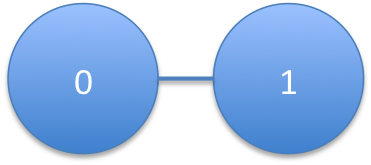
\includegraphics[scale=1]{1d_hypercube}
\end{center}
\end{frame}
\begin{frame}[fragile]
  \frametitle{Visualizing 6D Hypercube}
Here is the second dimension!\\
Note that there are two edges per node.
\begin{center}
  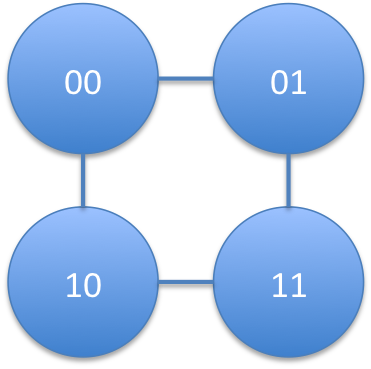
\includegraphics[scale=1]{2d_hypercube}
\end{center}
\end{frame}
\begin{frame}[fragile]
  \frametitle{Visualizing 6D Hypercube}
Here is the third dimension!\\
Note that there are three edges per node.\\
Here, instead of spreading to our conventional three dimensional space, let's visualize it in just a 2D space still, where we just have edge crossing over between left end and right end.\\
\begin{center}
  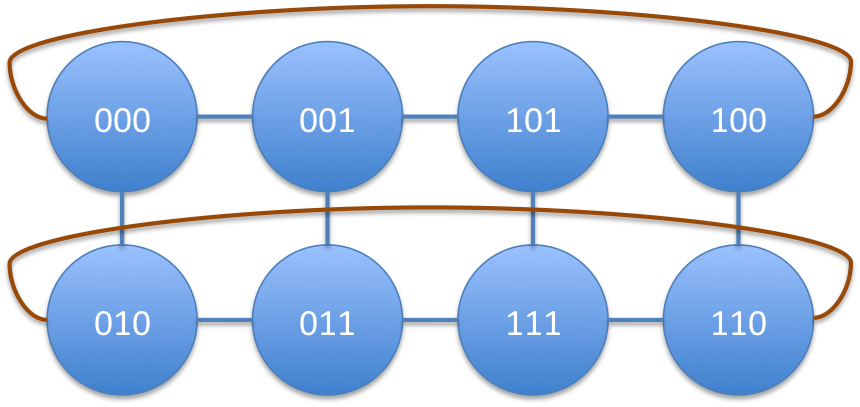
\includegraphics[scale=.5]{3d_hypercube}
\end{center}
\end{frame}
\begin{frame}[fragile]
  \frametitle{Visualizing 6D Hypercube}
Here is the fourth dimension!\\
Note that there are four edges per node.\\
If you notice with the three dimension one, there is still one side on each node that is not used, right? So we can make use of that spot to spread to four dimensions in just 2D visual space.
\begin{center}
  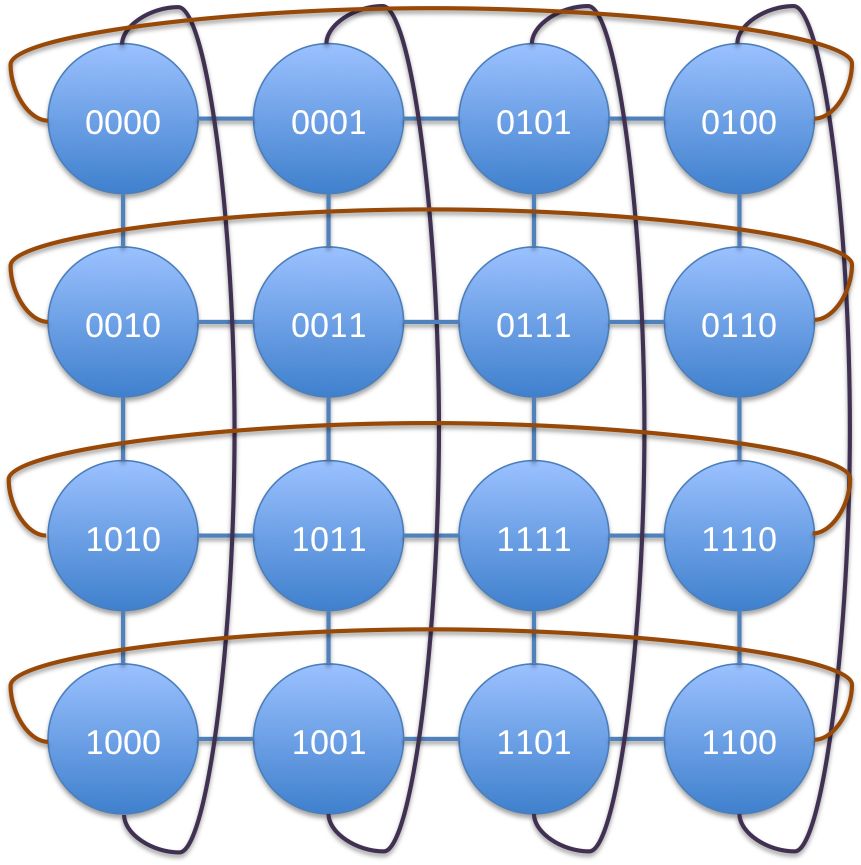
\includegraphics[scale=.25]{4d_hypercube}
\end{center}
\end{frame}
\begin{frame}[fragile]
  \frametitle{Visualizing 6D Hypercube}
Now in the previous 2D virtual space, there is no more sides to make use of, right? Because of that, NOW we move onto 3D virtual space to try showing higher dimension. To go further, imagine that the 4D hypercube graph you saw earlier turned sideways. (Literally, move the paper 90 degrees).\\
\begin{center}
  
\includegraphics[scale=.25]{4d_hypercube_side}
\end{center}
\end{frame}
\begin{frame}[fragile]
  \frametitle{Visualizing 6D Hypercube}
You can see how there are still two sides on each circle that haven't been used yet, right? We can make use of one of them to get us to visualize 5D hypercube!\\
\begin{center}
  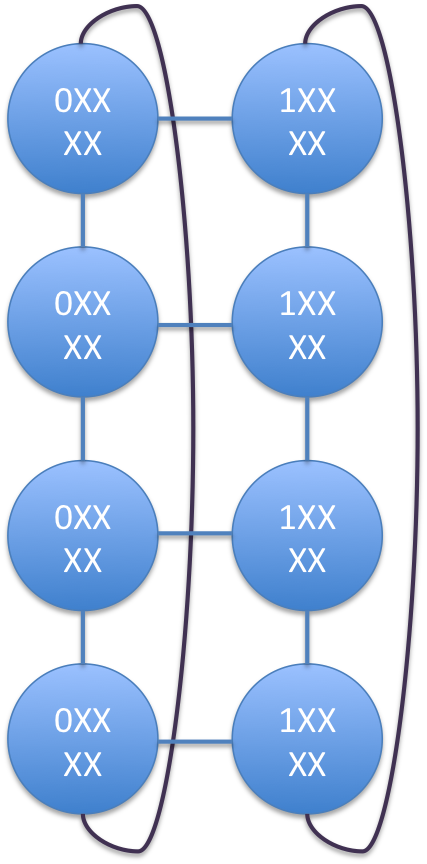
\includegraphics[scale=.25]{5d_hypercube}
\end{center}
\end{frame}
\begin{frame}[fragile]
  \frametitle{Visualizing 6D Hypercube}
Now lastly, we make use of one more side left on the circle, and by filling that side, we have reached 6D hypercube.\\
\begin{center}
  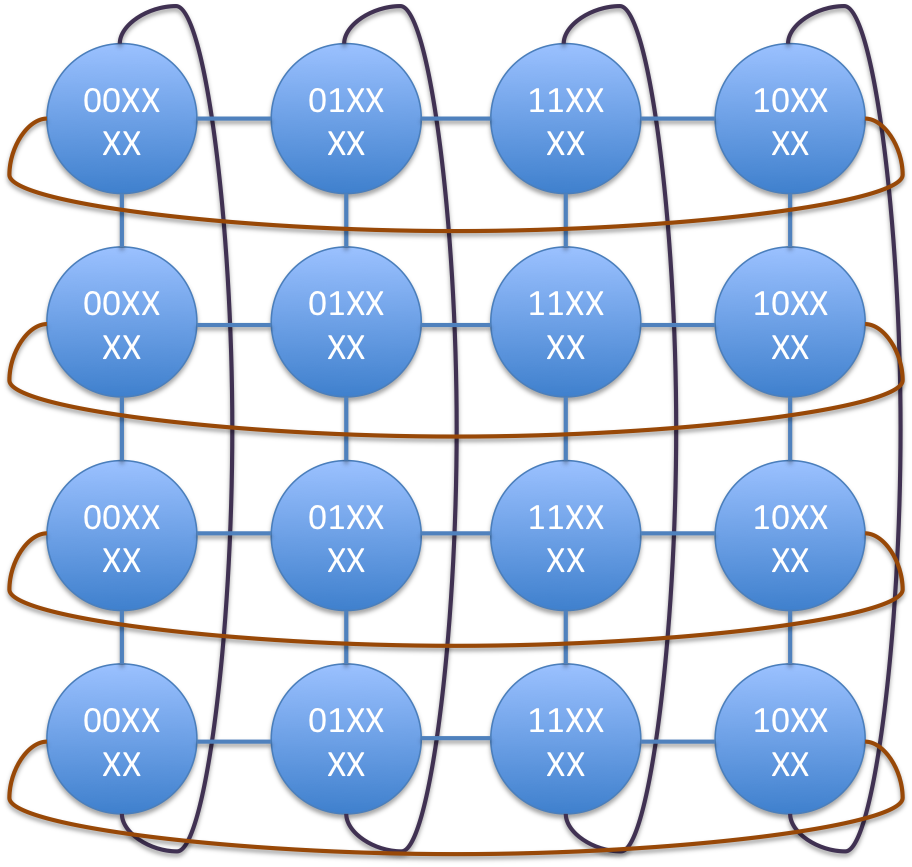
\includegraphics[scale=.25]{6d_hypercube}
\end{center}
\end{frame}
\begin{frame}[fragile]
  \frametitle{Visualizing 6D Hypercube}
That might have been a bit difficult, but I hope it wasn't too hard to understand? To put it in perspective of what we just visualized, here is how the full 6D hypercube would look to us at an angle!
\begin{center}
  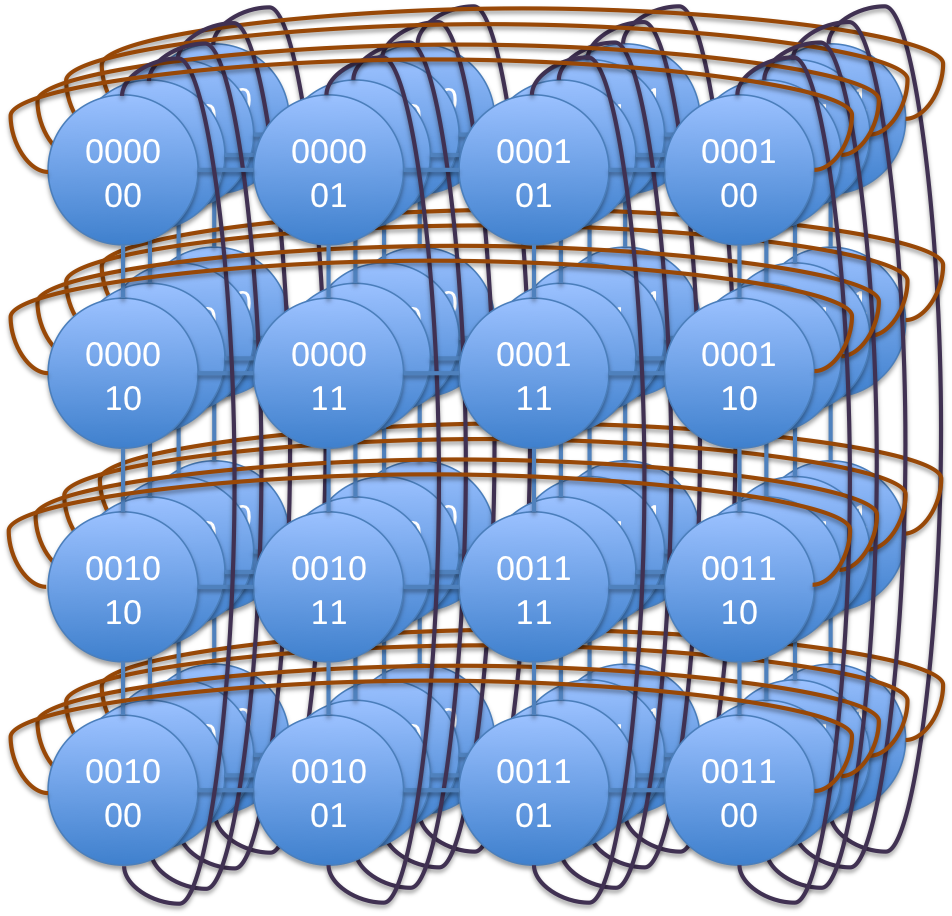
\includegraphics[scale=.25]{6d_hypercube_full}
\end{center}
\end{frame}

\begin{frame}[fragile]
  \frametitle{Complete Graphs}
Wikipedia: ``A \textbf{complete} graph is an undirected graph in which every pair of distinct vertices is connected by a unique edge.''
\begin{enumerate}[(a)]
\item How many edges are in a complete graph with 100 nodes? \uncover<2->{\alert<2>{ $\frac{100 \cdot 99}{2}$ }}
\item Does an Eulerian path exist such a graph? \uncover<3->{\alert<3>{ No }}
\item Does an Eulerian cycle exist in such a graph? \uncover<3->{\alert<3>{ No }}
\item Does a Hamiltonian path exist in such a graph? \uncover<4->{\alert<4>{ Yes }}
\item Does a Hamiltonian cycle exist in such a graph? \uncover<4->{\alert<4>{ Yes }}
\end{enumerate}
\end{frame}

\begin{frame}[fragile]
  \frametitle{Complete Graphs (cont.)}
Now we generate a complete graph with 101 nodes. Then we remove 1 randomly chosen edge.
\begin{enumerate}[(a)]
\item Does an Eulerian path exist in this graph?  \uncover<2->{\alert<2>{ Yes }}
\item Does an Eulerian cycle exist in this graph?  \uncover<3->{\alert<3>{ No }}
\item \uncover<3->{Now, what is the minimum number of edges you need to remove additionally to make this graph have an Eulerian cycle?}  \uncover<4->{\alert<4>{ 2 }}
\end{enumerate}
\end{frame}

\begin{frame}[fragile]
  \frametitle{Hypercube Question}
\begin{enumerate}[(a)]
\item If you have degree 4 hypercube and you remove one edge from it, does it have an Eulerian cycle? \uncover<2->{\alert<2>{No}}
\item \uncover<2->{In that case, what is the minimum number of edges you need to remove additionally to make this graph have an Eulerian cycle?} \uncover<3->{\alert<3>{3}}
\end{enumerate}
\end{frame}


% Counting/Discrete Probability %
% ---------------------------------------------------------------------------- %
\section{Counting}
  \subsection{Counting}

\begin{frame}[fragile]
  \frametitle{Counting Words}
\begin{enumerate}[(a)]
\item How many 7 letter words can be spelled with the 7 letters ``abcdefg'' without repeating any letter?
\uncover<2->{\alert<2>{7! = 5040}} \\ \vspace{5.0mm}
\item How many 4 letter words can be spelled with the 7 letters ``abcdefg'' without repeating any letter?
\uncover<3->{\alert<3>{$\frac{7!}{3!} = 840$}} \\ \vspace{5.0mm}
\item How many 4 letter words can you spell with 2 A's and 2 B's?
\uncover<4->{\alert<4>{$\frac{4!}{2!} / 2! = 6$}}
\end{enumerate}
\end{frame}

\begin{frame}[fragile]
  \frametitle{Two-Headed Monster}
\begin{enumerate}[(a)]
\item When tossing 4 coins, what is the probability of getting exactly 2 heads?
\uncover<2->{\alert<2>{$\frac{3}{8}$}} \\ \vspace{5.0mm}
\item When tossing 4 coins, what is the probability of getting at least 2 heads?
\uncover<3->{\alert<3>{$\frac{11}{16}$}}
\end{enumerate}
\end{frame}

\begin{frame}[fragile]
  \frametitle{Playing with Dice}
\begin{enumerate}[(a)]
\item When rolling 2 dice, what is the probability of snake eyes (i.e. two 1's)?
\uncover<2->{\alert<2>{$\frac{1}{36}$}}\\ \vspace{5.0mm}
\item When rolling 2 dice, what is the probability of getting one 1 and one 2?
\uncover<3->{\alert<3>{$\frac{1}{18}$}}\\ \vspace{5.0mm}
\item When rolling 4 dice, what is the probability of getting four 1's?
\uncover<4->{\alert<4>{$\frac{1}{6^4} = \frac{1}{1296}$}}\\ \vspace{5.0mm}
\item When rolling 4 dice, what is the probability of getting two 1's and two 3's?
\uncover<5->{\alert<5>{$(\frac{1}{6^4}) \cdot 6 = \frac{1}{6^3} = \frac{1}{216}$}}
\end{enumerate}
\end{frame}

% Conditional Probability %
% ---------------------------------------------------------------------------- %
\section{Conditional Probability}
  \subsection{Conditional Probability}

\begin{frame}
  \frametitle{Bayesian Inference Basics}
Let's say you are given Pr[A], $Pr[B|A]$, and $Pr[B|\overline{A}]$. How do you find $Pr[A|B]$?
\uncover<2->{
\begin{align}
Pr[A|B] &= \frac{Pr[A \cap B]}{Pr[B]}\\
Pr[B|A] = \frac{Pr[A \cap B]}{Pr[A]} &\Rightarrow Pr[A \cap B] = \frac{Pr[B|A]}{Pr[A]}\\
Pr[B] = Pr[A \cap B] + Pr[\overline{A} \cap B] &= Pr[B|A]Pr[A] + Pr[B|\overline{A}](1-Pr[A])\\
Pr[A|B] &= \frac{Pr[B|A]Pr[A]}{Pr[B|A]Pr[A] + Pr[B|\overline{A}](1-Pr[A])}
\end{align}
Line 2 refers to Baye's Rule and line 3 refers to the Total Probability Rule.\\
}
\end{frame}

\begin{frame}[fragile]
  \frametitle{Am I Crazy?}
Chris wants to know if he has bipolar disorder. Let $C$ be the event that Chris has bipolar disorder. The incidence of bipolar disorder in the general population is 1\%. He is really poor, so he asks his older brother Alex to make his diagnosis. If someone has bipolar disorder, Alex correctly identifies it 80\% of the time, but if someone does not have bipolar disorder, Alex makes a false accusation of bipolar 30\% of the time. Let $A$ be the event that Alex diagnoses Chris of having bipolar disorder. Assume $Pr[C]$ = 0.01. \\
\begin{enumerate}[(a)]
\uncover<2->{\item Find $Pr[A|C]$ }
\uncover<3->{\alert<3>{ 0.8 (Read this straight from problem statement)}}\\ 
\uncover<2->{\item Find $Pr[A]$}
\uncover<4->{\alert<4>{$= Pr[A|C] \cdot Pr[C] + Pr[A|\bar{C}] \cdot Pr[\bar{C}]$ \\
= $(0.8)\cdot (.01) + (0.3) \cdot (1 - .01) = 0.305$ }}\\ 
\uncover<2->{\item Find $Pr[C|A]$ (The probability that Chris has bipolar disorder given that Alex diagnoses him with bipolar disorder). }
\uncover<5->{\alert<5>{$= \frac{Pr[A|C]\cdot Pr[C]}{Pr[A]} = \frac{0.8 \cdot 0.01}{0.305} = \frac{8}{305}$ }}\\
\uncover<2->{\item Let $B$ be the event that Chris receives a correct diagnoses from Alex. Find $Pr[B]$ }\\
\uncover<6->{\alert<6>{
$= Pr[A \cap C] + Pr[\bar{A} \cap \bar{C}]$\\
$= Pr[A|C] \cdot Pr[C] + Pr[\bar{A}|\bar{C}] \cdot Pr[\bar{C}] = 0.701$
}}
\end{enumerate}
\end{frame}

\begin{frame}
  \frametitle{Am I Crazy? (cont.)}
\begin{enumerate}[(a)]
\setcounter{enumi}{4}
\item Let's generalize the answer to (d). Let $D$ be the event that a psychologist diagnoses Chris as having bipolar disorder. $Pr[D|C] = p$ and $Pr[D|\neg C] = q$. Let $Pr[C] = s$. Let $B'$ be the event that Chris receives a correct diagnosis from the psychologist. \\
\begin{enumerate}[i]
\uncover<2->{\item Find $Pr[B'].$ }
\uncover<3->{\alert<3>{ $sp+(1-s)(1-q)$ }}\\ \vspace{5.00mm}
\uncover<2->{\item What is the effect of raising p? (Does this make intuitive sense?) }\\
\uncover<4->{\alert<4>{ Increases accuracy of diagnosis }}\\ \vspace{5.00mm}
\uncover<2->{\item What is the effect of raising q? (Does this make intuitive sense?) }\\
\uncover<5->{\alert<5>{ Decreases accuracy of diagnosis }}\\ \vspace{5.00mm}
\uncover<2->{\item What is the effect of raising s? (Why is this the case?) }\\
\uncover<6->{\alert<6>{ It depends... }}
\end{enumerate}
\end{enumerate}
\end{frame}




\begin{frame}
  \frametitle{Bayesian Inference}
There are three indistinguishable boxes. One of them has 2 prize balls out of 10, another one has 4 prize balls out of 10, and the last one has 0 prize balls out of 10. The previous contestant chose from a random box and drew a prize ball out. What is the probability that he drew from the box with 2 prize balls given that he drew a prize ball?
\uncover<2->{\alert<2>{\\
Let $A$ = event that the chosen box has 2 prizes. \\
Let $B$ = event that the previous contestant got a prize ball.
\begin{align*}
Pr[A] &= 1/3\\
Pr[B | A] &= .2\\
Pr[B| \neg A] &= .2\\
Pr[A | B] &= \frac{Pr[B | A]Pr[A ]}{Pr[B| A]Pr[A] + Pr[B| \neg A](1-Pr[A])}\\
Pr[A| B] &= \frac{0.2 * 0.33}{0.2 * 0.33 + 0.2 * 0.67}\\
Pr[A| B] &= 0.33
\end{align*}
}}
\end{frame}


\begin{frame}
  \frametitle{More Bayesian Inference}
Since the previous contestant just drew a prize ball, Now, there are 9 balls in that box, while the other boxes still have 10 balls. To get the best chance of obtaining a prize ball, should you select that box? Or try choosing from one of the other two boxes?\\
\uncover<2->{\alert<2>{\small{
First, you need to find the probability that the previous contestant chose the 4 prizes box.

Let $C$ = event that the chosen box has 4 prizes.\\
Let $B$ = event that the previous contestant got a prize ball.
\begin{align*}
Pr[C] &= 1/3\\
Pr[B| C] &= .4\\
Pr[B | \neg C] &= .1\\
Pr[C | B] &= \frac{Pr[B| C]Pr[C]}{Pr[B| C]Pr[C] + Pr[B| \neg C](1-Pr[C])}\\
Pr[C| B] &= \frac{0.4 * 0.33}{0.4 * 0.33 + 0.1 * 0.67}\\
Pr[C| B] &= 0.67
\end{align*}
}}}
\uncover<3->{\alert<3>{
\small{Or if you aren't silly like me, you could have just seen that the probability of it being 4 prizes given someone got a prize from there is just $1 - Pr[\text{chosen box has 2 prizes} | \text{previous contestant got a prize}]$.}\\
}}
\end{frame}

\begin{frame}
  \frametitle{More Bayesian Inference (cont.)}
Since the previous contestant just drew a prize ball, Now, there are 9 balls in that box, while the other boxes still have 10 balls. To get the best chance of obtaining a prize ball, should you select that box? Or try choosing from one of the other two boxes?\\
\alert<1>{
Now that you have that information, you can get the expected value of drawing from that box or drawing from one of the other boxes. Let's say the box that the last contestant drew from is called Q.\\

Let $A$ = event that Q has 2 prizes. \\
Let $B$ = event that the previous contestant got a prize. \\
Let $C$ = event that Q has 4 prizes.\\
Let $D$ = event that you win a prize by drawing from Q. \\
Let $E$ = event that you win a prize by drawing from the other box.
\begin{align*}
Pr[D] &= Pr[A | B] * 1/9 + Pr[C | B] * 3 / 9 \\
Pr[D] &= 0.26\\
Pr[E] &= Pr[A | B] * 0.5 * 0.4 + Pr[C | B] * 0.5*0.2\\
Pr[E]  &= 0.13
\end{align*}
}
\end{frame}


% Hashing %
% ---------------------------------------------------------------------------- %
\section{Hashing}
\subsection{Hashing}

\begin{frame}[fragile]
  \frametitle{Hashing Collision Probability}
{\small What is the largest number, $m$, of keys we can store before the probability of a collision reaches $p$? \\ \vspace{5.0mm}
\uncover<2->{How can we approach this problem?}\\ \vspace{5.0mm}
\uncover<3->{\textbf{Step 1: } Express the problem formally.}\\ \vspace{5.0mm}
\uncover<4->{Notice that Pr[collision] $\leq p \equiv$ Pr[no collision] $\geq p$\\ \vspace{5.0mm}
It's much easier to express the probability of no collisions! Let's define this formally as:\\ \vspace{5.0mm}

Event A: Event that there are no collisions in a hash table with $m$ items and $n$ buckets.}

}

\end{frame}
\begin{frame}[fragile]
  \frametitle{Computing Pr[A]}

Let's assume $ m \leq n$. Otherwise, the probability that there are $m$ non-colliding objects in $n$ buckets is trivially zero.\\ \vspace{5.0mm}
\uncover<2->{We can think of this as a balls and bins problem! We simply want to throw $m$ balls into $n$ bins and calculate the probability that none of the balls collide.}

\uncover<3->{\begin{align*}
Pr[A] = &Pr(\texttt{first ball doesn't collide}) \cdot Pr(\texttt{second ball doesn't collide}) \\
      & \cdot ... \cdot Pr(\texttt{mth ball doesn't collide})\\
= &\frac{n}{n} \cdot \frac{n-1}{n} \cdot ... \cdot \frac{n-(m-1)}{n}
\end{align*}}

\end{frame}

\begin{frame}[fragile]
  \frametitle{Here Comes the Math}
Let's begin by taking the natural log of both sides.
\uncover<2->{
$$
ln(Pr[A]) = ln(1 - \frac{1}{n}) + ln(1 - \frac{2}{n}) + ... + ln(1 - \frac{m-1}{n})
$$
}
\uncover<3->{Next, we're going to use the approximation $ln(1 - x) \approx -x$ if x is small.}

\uncover<4->{Rewriting our expression:

\begin{align*}
ln(Pr[A]) &\approx -\frac{1}{n} - \frac{2}{n} - ... - \frac{m-1}{n}\\
&= - \frac{1}{n} \sum_{i=1}^{m-1} i\\
&= - \frac{1}{n} \cdot \frac{m(m-1)}{2}\\
&\approx - \frac{m^2}{2n}
\end{align*}
}

\uncover<5->{Let's do a little more math...
$$
Pr[A] \approx e^{- \frac{m^2}{2n}}
$$
}
\end{frame}

\begin{frame}[fragile]
  \frametitle{Solving for m}
So far we have:
$$
Pr[A] \approx e^{- \frac{m^2}{2n}}
$$
\uncover<2->{This whole time, we've been trying to solve for Pr[A] $\geq$ p . So let's plug in and solve!
\begin{align*}
Pr[A] &\approx e^{- \frac{m^2}{2n}} \geq p\\
&- \frac{m^2}{2n} \geq ln(p) \\
&m \leq \sqrt{2n \cdot ln(1/p)}
\end{align*}
}
\end{frame}

\begin{frame}[fragile]
  \frametitle{Bringing It All Together}
\begin{enumerate}[(a)]
\item What assumptions/approximations are made in the derivation we just went through?\\
\uncover<2->{
\begin{itemize}
\item[1.] Assumed $m \leq n$.
\item[2.] $ln(1 - x) \approx -x$ when x is small
\item[3.] Assumed x is small
\item[4.] Approximated $\frac{m(m-1)}{2n} \approx \frac{m^2}{2n}$
\end{itemize}
}
\item If we halved the size of the hash table, how would the collision probability change? Recall $m \leq \sqrt{2n  \cdot ln(1/p)}$.\\
\uncover<3->{Solving for p as a function of $m$ and $n$:\\
$$
p \leq e^{- \frac{m^2}{2n}}
$$
If $n$ is halved, the exponent doubles. Then, we could write:
\begin{align*}
p_{new} \leq e^{- \frac{2m^2}{2n}} &= (e^{- \frac{m^2}{2n}})^2 \\
&= p_{old}^2
}
\end{align*}
\end{enumerate}
\end{frame}


\end{document}
